\section{Context}
Our application targets a work environment or an educational environment.
%The targeted environment is all work or educational environment.
The analysis and design process is based upon a university, but the application is easily implemented at any other work environment. 

\begin{figure}[ht]%
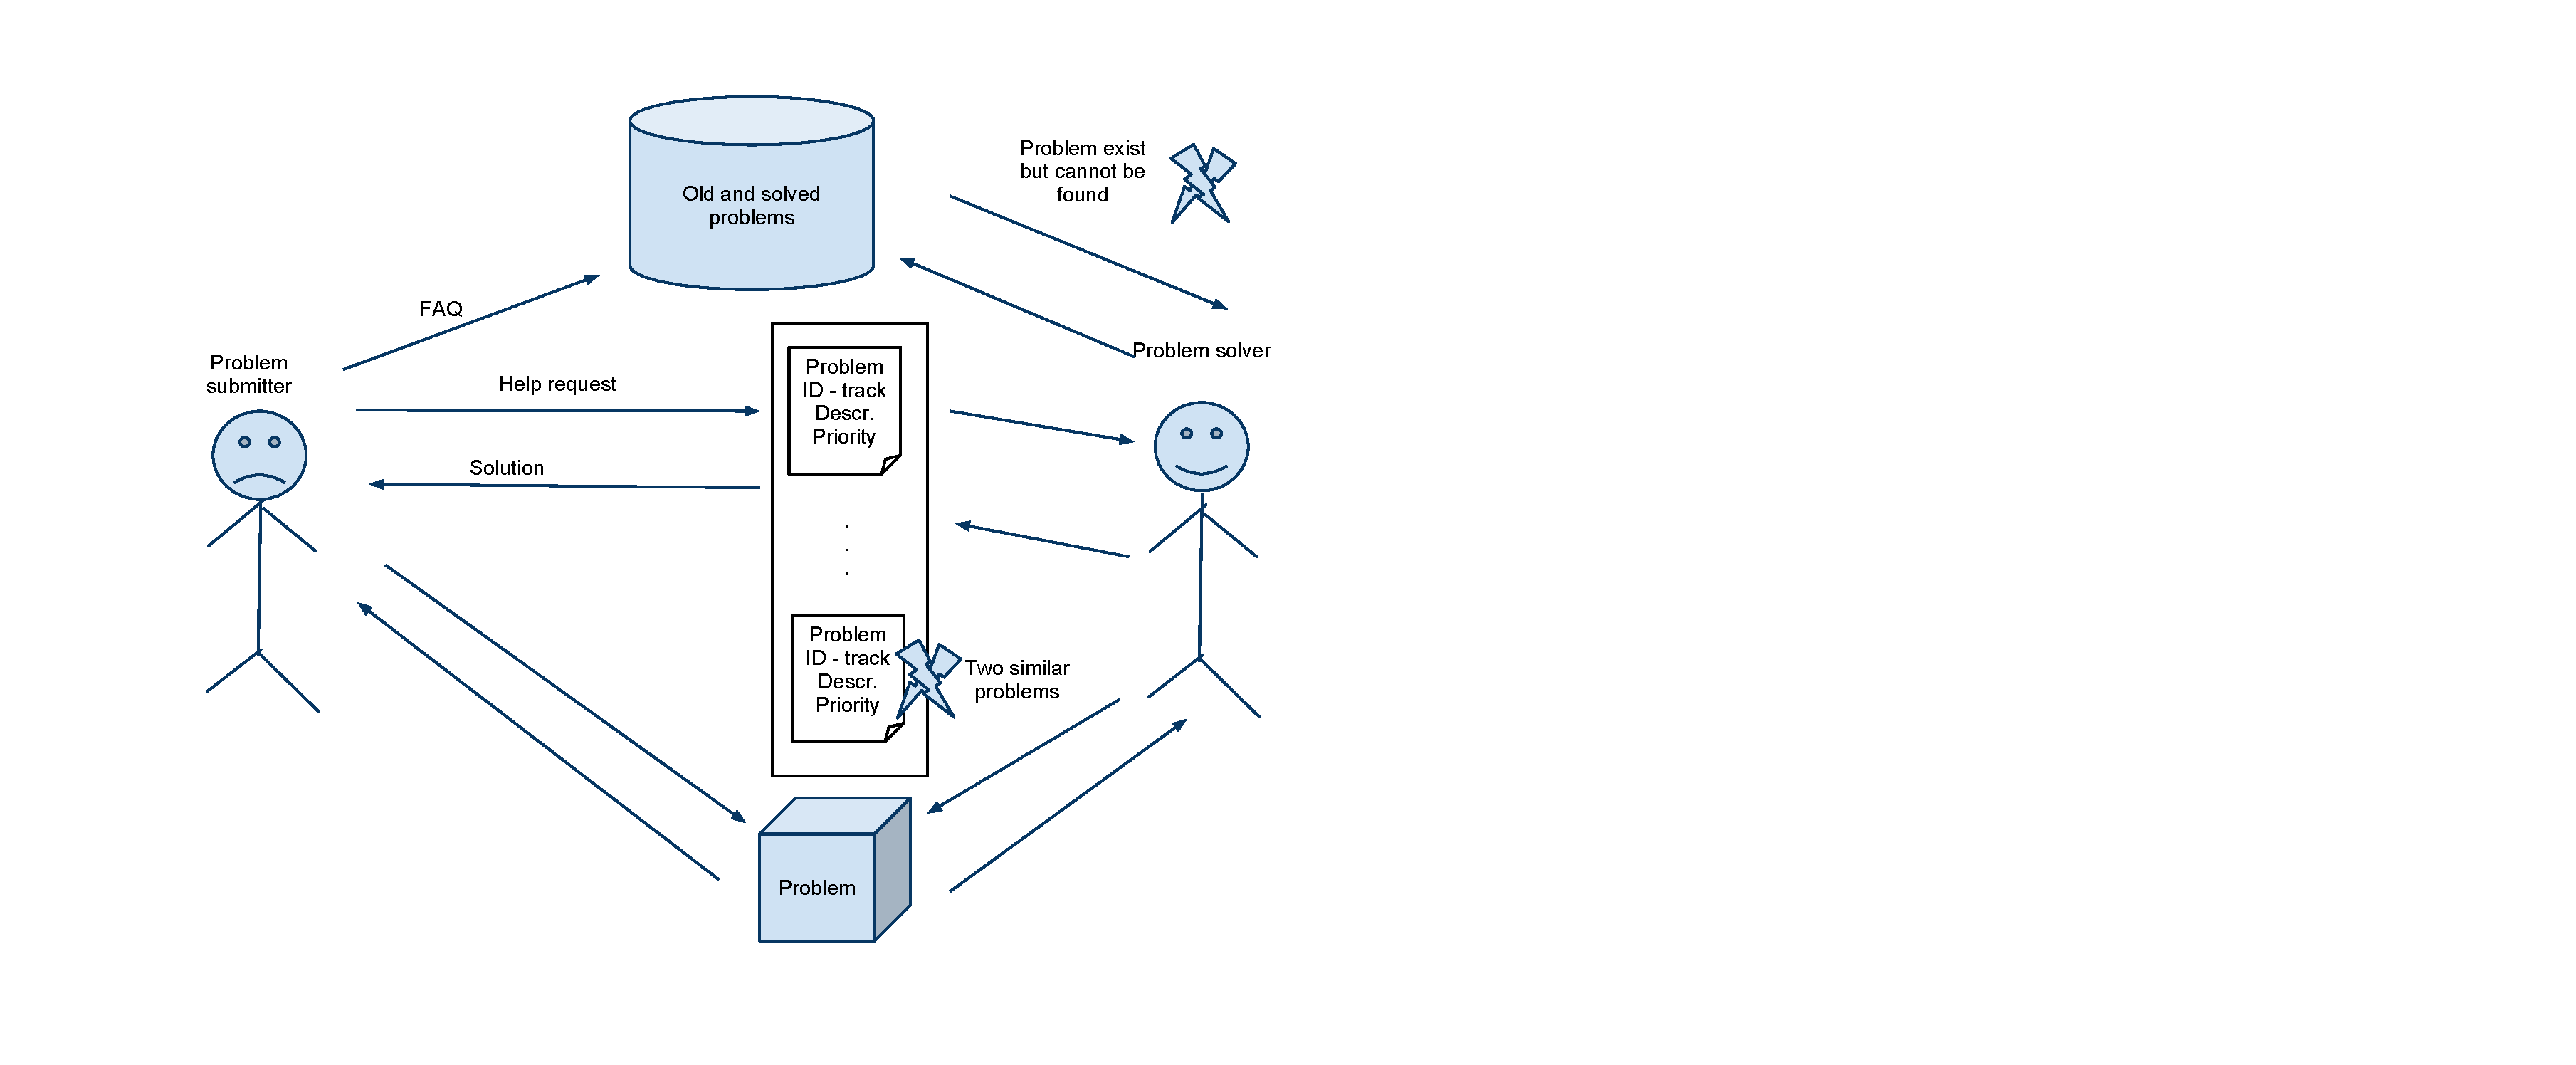
\includegraphics[scale = 0.42]{input/background/rich_picture.pdf}%
\morscaption{Rich picture of our application}%
\label{fig:rich_picture}%
\end{figure}

To fully understand the context we draw a rich picture which can be seen on figure \ref{fig:rich_picture}. 
The central aspects of the rich picture is that both the problem submitter and the problem solver can act on the problem, and will communicate through the application. 
From the rich picture we see a few conflicts in the environment:
\begin{itemize}
		\item The first is that problem exist but cannot be found.
		\item The second is that there could exist two similar problem.
		\item The central objects in the application are the problems and solutions.
\end{itemize} 
\vspace{-3mm}
\subsection{Problem Domain}
A central phenomena in our application is to add a problem to the application.
This will occur when a \aclient[] finds a problem in the organization/institution and wants to submit it, in order to get it solved.
%This phenomena will also include a staff member, namely the one who will initially be assigned to the problem.

Another important phenomena in our application is when a problem is solved.
This is initiated by a staff member and will result in a notification to the \aclient s who are subscribing to alterations of the problem, for example solutions or comments being added.
%A client who submit the problem can suggest it to be reopened if he/she is not satisfied with the solution.

Chapter \ref{chap:problemDomain} gives a detailed analysis of the problem domain and will elaborate on the phenomena.
\vspace{-3mm}
\subsection{Application Domain}
The people who will be acting on the application are the problem solver and submitter. Most likely the submitter will be a student in a university environment and the solver will be the technical staff member. But the submitter could be a staff member as well. Beside the two main actors there is an admin who can administrate the staff, clients, and the application itself.

A detailed analysis of the application domain is presented in chapter \ref{chap:app_domain}, where the actors and their use cases are further described.